% Options for packages loaded elsewhere
\PassOptionsToPackage{unicode}{hyperref}
\PassOptionsToPackage{hyphens}{url}
\PassOptionsToPackage{dvipsnames,svgnames,x11names}{xcolor}
%
\documentclass[
  letterpaper,
  DIV=11,
  numbers=noendperiod]{scrartcl}

\usepackage{amsmath,amssymb}
\usepackage{iftex}
\ifPDFTeX
  \usepackage[T1]{fontenc}
  \usepackage[utf8]{inputenc}
  \usepackage{textcomp} % provide euro and other symbols
\else % if luatex or xetex
  \usepackage{unicode-math}
  \defaultfontfeatures{Scale=MatchLowercase}
  \defaultfontfeatures[\rmfamily]{Ligatures=TeX,Scale=1}
\fi
\usepackage{lmodern}
\ifPDFTeX\else  
    % xetex/luatex font selection
\fi
% Use upquote if available, for straight quotes in verbatim environments
\IfFileExists{upquote.sty}{\usepackage{upquote}}{}
\IfFileExists{microtype.sty}{% use microtype if available
  \usepackage[]{microtype}
  \UseMicrotypeSet[protrusion]{basicmath} % disable protrusion for tt fonts
}{}
\makeatletter
\@ifundefined{KOMAClassName}{% if non-KOMA class
  \IfFileExists{parskip.sty}{%
    \usepackage{parskip}
  }{% else
    \setlength{\parindent}{0pt}
    \setlength{\parskip}{6pt plus 2pt minus 1pt}}
}{% if KOMA class
  \KOMAoptions{parskip=half}}
\makeatother
\usepackage{xcolor}
\setlength{\emergencystretch}{3em} % prevent overfull lines
\setcounter{secnumdepth}{-\maxdimen} % remove section numbering
% Make \paragraph and \subparagraph free-standing
\ifx\paragraph\undefined\else
  \let\oldparagraph\paragraph
  \renewcommand{\paragraph}[1]{\oldparagraph{#1}\mbox{}}
\fi
\ifx\subparagraph\undefined\else
  \let\oldsubparagraph\subparagraph
  \renewcommand{\subparagraph}[1]{\oldsubparagraph{#1}\mbox{}}
\fi


\providecommand{\tightlist}{%
  \setlength{\itemsep}{0pt}\setlength{\parskip}{0pt}}\usepackage{longtable,booktabs,array}
\usepackage{calc} % for calculating minipage widths
% Correct order of tables after \paragraph or \subparagraph
\usepackage{etoolbox}
\makeatletter
\patchcmd\longtable{\par}{\if@noskipsec\mbox{}\fi\par}{}{}
\makeatother
% Allow footnotes in longtable head/foot
\IfFileExists{footnotehyper.sty}{\usepackage{footnotehyper}}{\usepackage{footnote}}
\makesavenoteenv{longtable}
\usepackage{graphicx}
\makeatletter
\def\maxwidth{\ifdim\Gin@nat@width>\linewidth\linewidth\else\Gin@nat@width\fi}
\def\maxheight{\ifdim\Gin@nat@height>\textheight\textheight\else\Gin@nat@height\fi}
\makeatother
% Scale images if necessary, so that they will not overflow the page
% margins by default, and it is still possible to overwrite the defaults
% using explicit options in \includegraphics[width, height, ...]{}
\setkeys{Gin}{width=\maxwidth,height=\maxheight,keepaspectratio}
% Set default figure placement to htbp
\makeatletter
\def\fps@figure{htbp}
\makeatother

\usepackage{booktabs}
\usepackage{longtable}
\usepackage{array}
\usepackage{multirow}
\usepackage{wrapfig}
\usepackage{float}
\usepackage{colortbl}
\usepackage{pdflscape}
\usepackage{tabu}
\usepackage{threeparttable}
\usepackage{threeparttablex}
\usepackage[normalem]{ulem}
\usepackage{makecell}
\usepackage{xcolor}
\usepackage[auth-lg]{authblk}
\KOMAoption{captions}{tableheading}
\makeatletter
\makeatother
\makeatletter
\makeatother
\makeatletter
\@ifpackageloaded{caption}{}{\usepackage{caption}}
\AtBeginDocument{%
\ifdefined\contentsname
  \renewcommand*\contentsname{Table of contents}
\else
  \newcommand\contentsname{Table of contents}
\fi
\ifdefined\listfigurename
  \renewcommand*\listfigurename{List of Figures}
\else
  \newcommand\listfigurename{List of Figures}
\fi
\ifdefined\listtablename
  \renewcommand*\listtablename{List of Tables}
\else
  \newcommand\listtablename{List of Tables}
\fi
\ifdefined\figurename
  \renewcommand*\figurename{Figure}
\else
  \newcommand\figurename{Figure}
\fi
\ifdefined\tablename
  \renewcommand*\tablename{Table}
\else
  \newcommand\tablename{Table}
\fi
}
\@ifpackageloaded{float}{}{\usepackage{float}}
\floatstyle{ruled}
\@ifundefined{c@chapter}{\newfloat{codelisting}{h}{lop}}{\newfloat{codelisting}{h}{lop}[chapter]}
\floatname{codelisting}{Listing}
\newcommand*\listoflistings{\listof{codelisting}{List of Listings}}
\makeatother
\makeatletter
\@ifpackageloaded{caption}{}{\usepackage{caption}}
\@ifpackageloaded{subcaption}{}{\usepackage{subcaption}}
\makeatother
\makeatletter
\@ifpackageloaded{tcolorbox}{}{\usepackage[skins,breakable]{tcolorbox}}
\makeatother
\makeatletter
\@ifundefined{shadecolor}{\definecolor{shadecolor}{rgb}{.97, .97, .97}}
\makeatother
\makeatletter
\makeatother
\makeatletter
\makeatother
\ifLuaTeX
  \usepackage{selnolig}  % disable illegal ligatures
\fi
\IfFileExists{bookmark.sty}{\usepackage{bookmark}}{\usepackage{hyperref}}
\IfFileExists{xurl.sty}{\usepackage{xurl}}{} % add URL line breaks if available
\urlstyle{same} % disable monospaced font for URLs
\hypersetup{
  pdftitle={Trabalho Prático 2},
  pdfauthor={Ana Tércia Freires da Silva -; Gabriel Véras Monteiro - 19/0106794; Gabriela Carneiro de Almeida - 18/0120816},
  colorlinks=true,
  linkcolor={blue},
  filecolor={Maroon},
  citecolor={Blue},
  urlcolor={Blue},
  pdfcreator={LaTeX via pandoc}}

\title{Trabalho Prático 2}
\usepackage{etoolbox}
\makeatletter
\providecommand{\subtitle}[1]{% add subtitle to \maketitle
  \apptocmd{\@title}{\par {\large #1 \par}}{}{}
}
\makeatother
\subtitle{Análise de Séries Temporais - 1/2023}
\author{Ana Tércia Freires da Silva - \and Gabriel Véras Monteiro -
19/0106794 \and Gabriela Carneiro de Almeida - 18/0120816}
\date{}

\begin{document}
\maketitle
\ifdefined\Shaded\renewenvironment{Shaded}{\begin{tcolorbox}[boxrule=0pt, enhanced, interior hidden, frame hidden, sharp corners, borderline west={3pt}{0pt}{shadecolor}, breakable]}{\end{tcolorbox}}\fi

\renewcommand*\contentsname{Table of contents}
{
\hypersetup{linkcolor=}
\setcounter{tocdepth}{3}
\tableofcontents
}
\newpage{}

\hypertarget{introduuxe7uxe3o-suxe9rie-selecionada-caracteruxedsticas-e-decomposiuxe7uxe3o}{%
\section{Introdução: série selecionada, características e
decomposição}\label{introduuxe7uxe3o-suxe9rie-selecionada-caracteruxedsticas-e-decomposiuxe7uxe3o}}

A série temporal escolhida foi a de número \emph{id} correspondente a
1891. De acordo com a definição do próprio pacote, refere-se a
\emph{Pneumatic casings, original equipment}. Foram realizadas medidas
mensais de 1982 a 1992 e o horizonte de previsão requerido é das 18
ocorrências seguintes.

O gráfico da série, com \emph{in} e \emph{out-sample}, é exposto a
seguir.

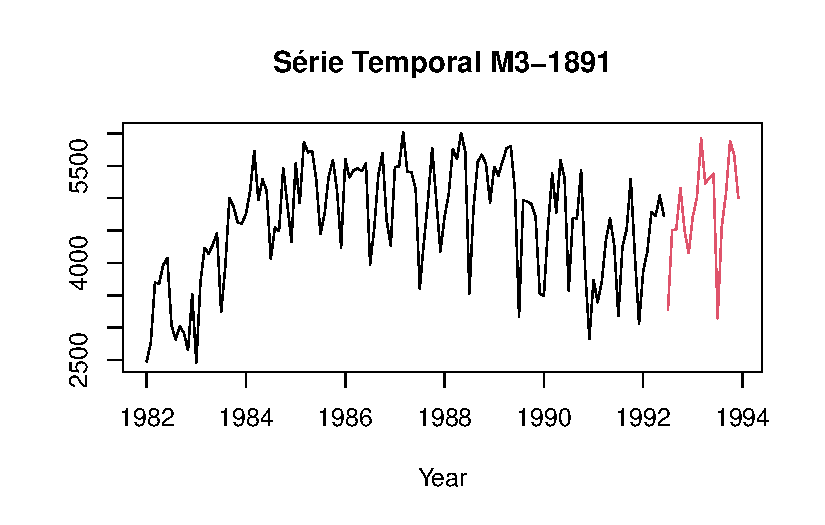
\includegraphics{T2_grupo10_files/figure-pdf/plot-serie-total-1.pdf}

Após visualização inical da série, foi feita sua decomposição via MSTL.
Foram feitas duas decomposições, uma ajustando \emph{lambda = ``auto''}
e \emph{lambda = NULL}, resultando em duas composições muito similares.

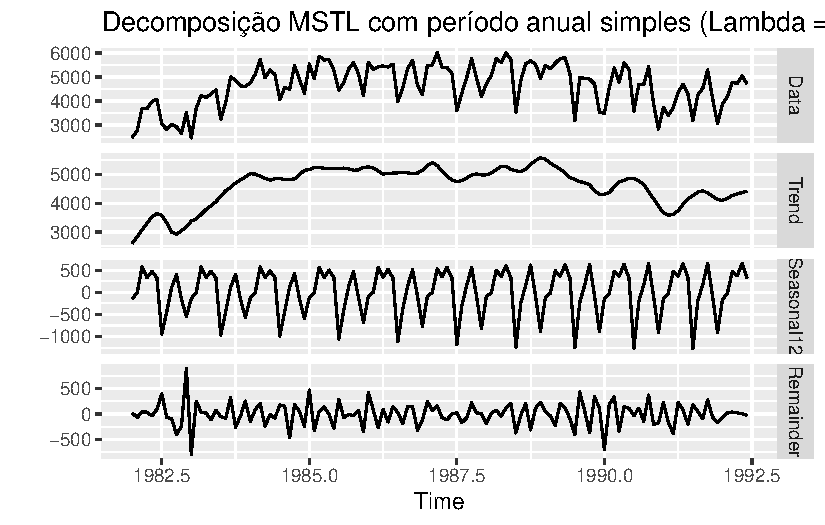
\includegraphics{T2_grupo10_files/figure-pdf/decomposicao-mstl-1.pdf}

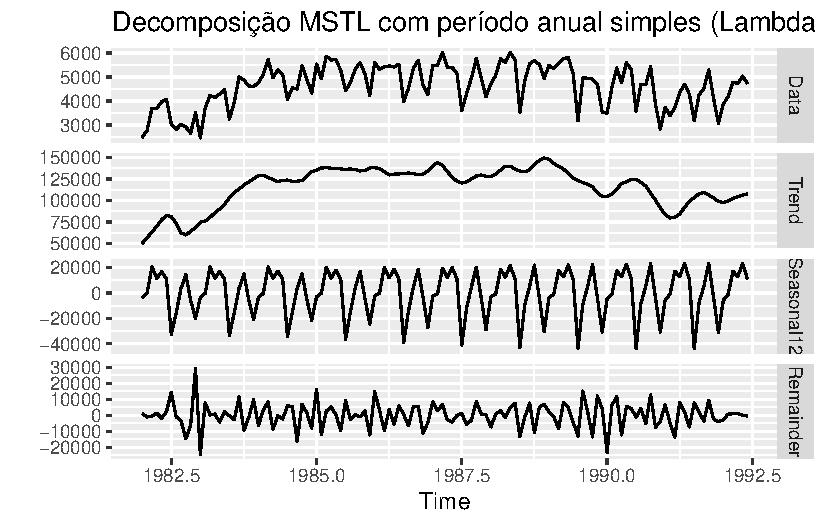
\includegraphics{T2_grupo10_files/figure-pdf/decomposicao-mstl-2.pdf}

Aplicando a decomposição MSTL com sazonalidade anual, é possível
visualizar uma tendência de crescimento no inicio das medições, passando
por uma estabilização e posterior decrescimento. Ao final, a série
parece retomar um pequeno crescimento. Além disso, é possível notar que
a série tem um componente sazonal mensal, com ciclos claros. Por fim, o
ruído parece se aproximar de um padãr de ruído branco.

\hypertarget{modelos-arima-seleuxe7uxe3o-transformauxe7uxf5es-e-resuxedduos}{%
\section{Modelos ARIMA: seleção, transformações e
resíduos}\label{modelos-arima-seleuxe7uxe3o-transformauxe7uxf5es-e-resuxedduos}}

\hypertarget{sem-transformauxe7uxe3o-de-box-cox}{%
\subsection{Sem transformação de
Box-Cox}\label{sem-transformauxe7uxe3o-de-box-cox}}

\begin{verbatim}

    KPSS Test for Level Stationarity

data:  serie_ms
KPSS Level = 0.52764, Truncation lag parameter = 4, p-value = 0.03544
\end{verbatim}

\begin{verbatim}
[1] 1
\end{verbatim}

\begin{verbatim}
[1] 1
\end{verbatim}

\begin{verbatim}

    KPSS Test for Level Stationarity

data:  serie_ms_diff
KPSS Level = 0.044309, Truncation lag parameter = 4, p-value = 0.1
\end{verbatim}

Inicialmente foi feito o teste de estacionaridade KPSS na série segundo
as hipóteses:

\begin{align}
  \begin{cases}
    H_0:\text{O processo é estacionário}\\
    H_1: \text{O processo possui raiz unitária}\\
  \end{cases}
\end{align}

O teste indica que a série não é estacionária (p-valor = 0,03544),
portanto, é necessário aplicar diferenciações para tornar a série
estacionária antes de ajustar um modelo adequado que se ajuste a série
em análise. O número de diferenciações simples necessárias é igual a um,
dessa forma, a estimativa para \emph{`d'} do modelo SARIMA é de
\emph{`d' = 1}. Além disso, em se tratanto de uma série sazonal, é
necessário verificar o número de diferenciações sazonais para retirar o
efeito da sazonalidade. Analogamente, foi obtido o valor de uma
diferenciação sazonal necessária, se tratando, portanto, do \emph{`D'}
do modelo SARIMA, sendo \emph{`D' = 1}. Para a diferenciação sazonal,
pelo ciclo sazonal ser igual a 12, é necessário a utilização do lag
sazonal igual a 12 (lag = 12).

\includegraphics{T2_grupo10_files/figure-pdf/grafico série diferenciada-1.pdf}

\begin{verbatim}

    KPSS Test for Level Stationarity

data:  serie_ms_diff
KPSS Level = 0.044309, Truncation lag parameter = 4, p-value = 0.1
\end{verbatim}

O gráfico acima mostra o comportamento da série após as diferenciações
simples e sazonal. A série aparenta ter comportamento estácionário, o
que foi confirmado a partir da aplicação do teste KPSS, cujas hipóteses
já foram explicitadas anteriormente. Por meio do teste foi possível
notar que a série realmente está estacionária após as diferenciações
(p-valor = 0,1), dessa forma, é possível proseguir com o procedimento de
seleção do modelo.

Para tal, se segue a análise dos gráficos ACF e PACF.

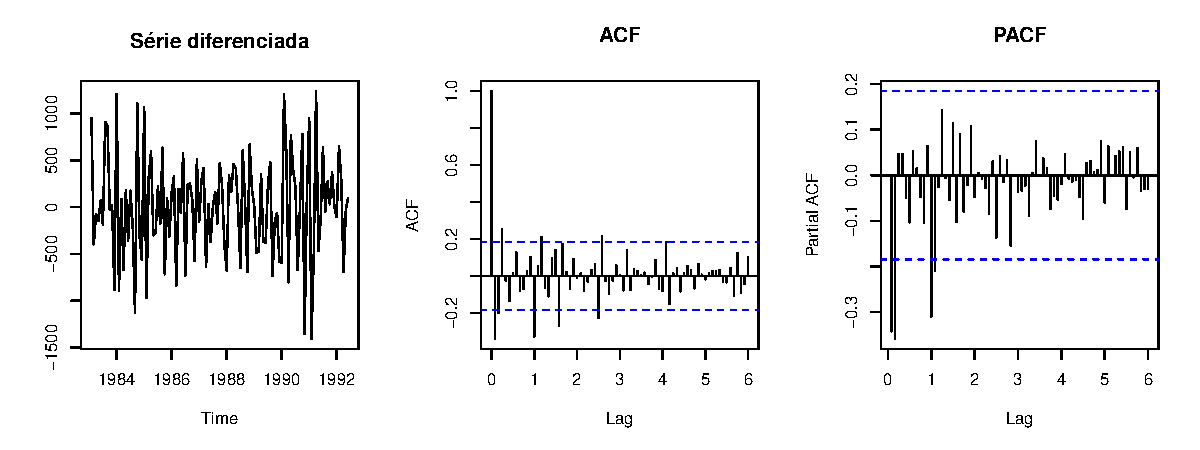
\includegraphics{T2_grupo10_files/figure-pdf/acf-pacf-sem-transformacao BoxCox-1.pdf}

É possível perceber que no ACF há uma quebra no primeiro lag simples, ao
passo que ocorre uma quebra no segundo lag do PACF. Porém, nenhum dos
gráficos apresenta comportamento bem definido, dificultando a
determinação do restante dos parâmetros do modelo SARIMA. Nesse
contexto, foi feito a combinação dos valores de \emph{p} e \emph{q},
entre 0 e 2, e de \emph{P} e \emph{Q}, nos valores 0 ou 1,
desconsiderando quando \emph{p} e \emph{q} fossem zero simultaneamente
e, analogamente, para \emph{P} e \emph{Q}. O melhor modelo, criado pelas
combinações de valores explicitados acima, foi selecionado segundo o
menor valor de AICc.

\begin{verbatim}
p = 0 , d = 1, q = 0 , P =  0 , D = 1, Q =  0 , AICc = 1750.899 
p = 0 , d = 1, q = 1 , P =  0 , D = 1, Q =  0 , AICc = 1729.316 
p = 0 , d = 1, q = 3 , P =  0 , D = 1, Q =  0 , AICc = 1729.225 
p = 1 , d = 1, q = 2 , P =  0 , D = 1, Q =  0 , AICc = 1729.027 
p = 2 , d = 1, q = 0 , P =  0 , D = 1, Q =  0 , AICc = 1724.938 
p = 0 , d = 1, q = 1 , P =  0 , D = 1, Q =  1 , AICc = 1709.211 
p = 2 , d = 1, q = 0 , P =  0 , D = 1, Q =  1 , AICc = 1706.182 
\end{verbatim}

\begin{verbatim}
[1] 1706.182
\end{verbatim}

A partir dos AICc, o modelo selecionado foi
\(SARIMA(2,1,0)(0,1,1)_{12}\), assim, pode-se prosseguir com a análise
dos resíduos.

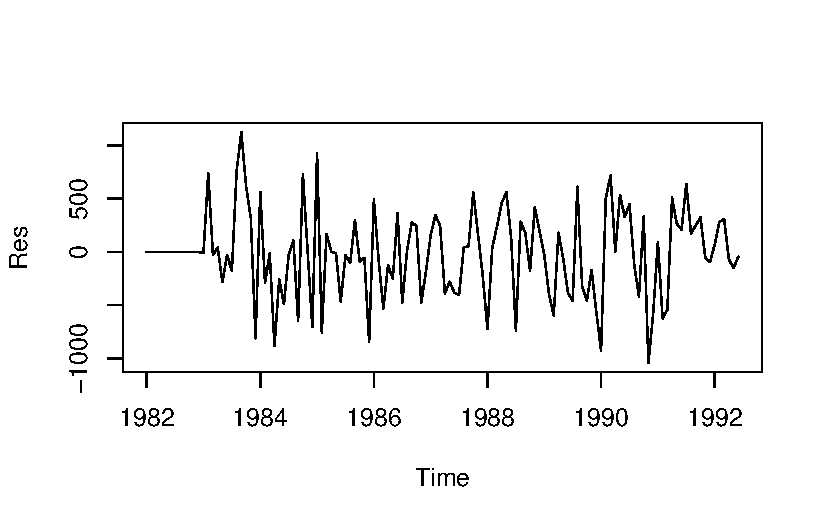
\includegraphics{T2_grupo10_files/figure-pdf/análise de resíduos - sem box-cox-1.pdf}

É notável que há uma sequência de resíduos iguais a zero no início da
série, e estes podem afetar as análises, dessa forma, os zeros foram
desconsiderados, sendo feita análise de resíduos de um ano após o início
da série, dados pela figura a seguir:

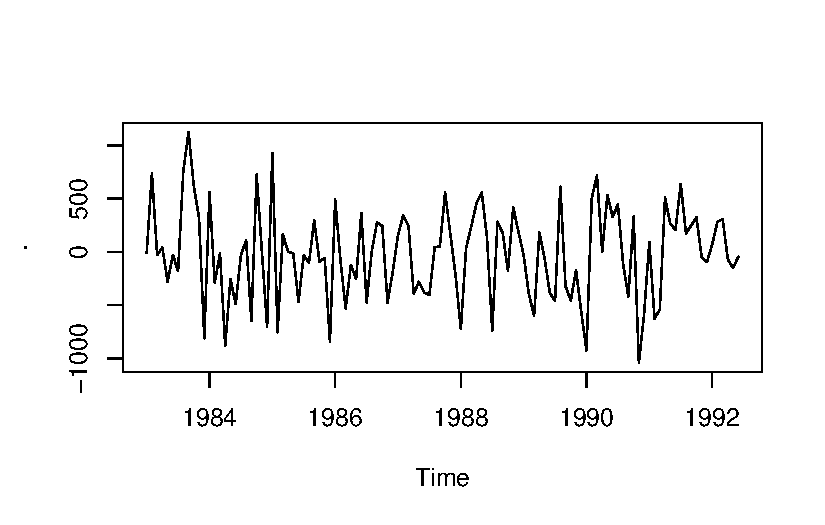
\includegraphics{T2_grupo10_files/figure-pdf/análise de resíduos - sem box-cox e sem zeros-1.pdf}

\begin{verbatim}

    KPSS Test for Level Stationarity

data:  E
KPSS Level = 0.062374, Truncation lag parameter = 4, p-value = 0.1
\end{verbatim}

Os resíduos aparentam ser estacionários, com média 0 e com variância
constante. Agora, foi testada a estacionariedade com um teste KPSS,
cujas as hipóteses já foram mencionadas. Como resultado, obtem-se que o
processo é estacionário (p-valor \textgreater{} 0, 1).

Além disso, a partir do gráfico do ACF, mostrado abaixo, pode-se
verificar a independência dos resíduos.

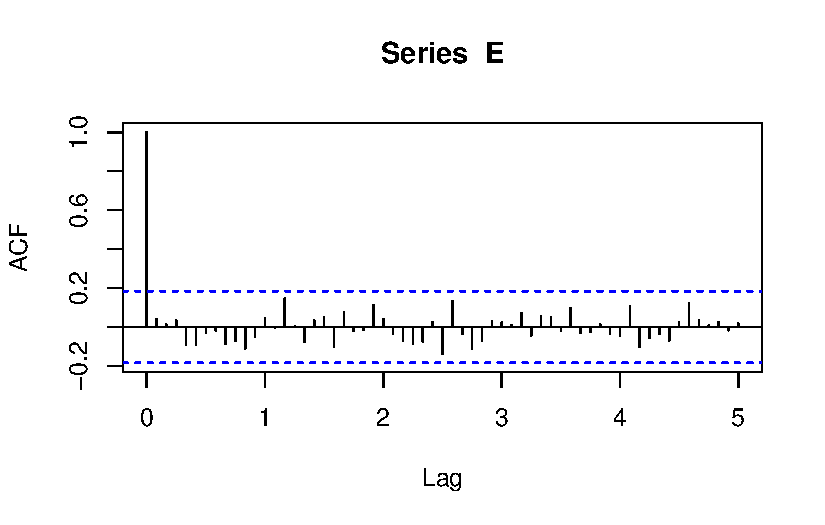
\includegraphics{T2_grupo10_files/figure-pdf/unnamed-chunk-1-1.pdf}

Observamos que praticamente todos os valores das autocorrelações não são
significantes, indicando a independência dos resíduos, o que necessita a
confirmação pelo teste de Ljung-Box, com base nas hipóteses:

\begin{align}
  \begin{cases}
    H_0:\text{Todas as correlações são iguais a zero}\\
    H_1: \text{Ao menos uma correlação é diferente de zero}\\
  \end{cases}
\end{align}

Assim, utilizando o teste com 20 graus de liberdade, obteve-se p-valor
de 0, 8923, e para 15, obteve-se 0, 8741, dessa maneira, utilizando o α
= 0, 05, não se rejeita H0, corroborando com a análise gráfica de que os
resíduos são independentes. Então, pode-se testar a normalidade,
primeiramente, por meio de uma representação gráfica.

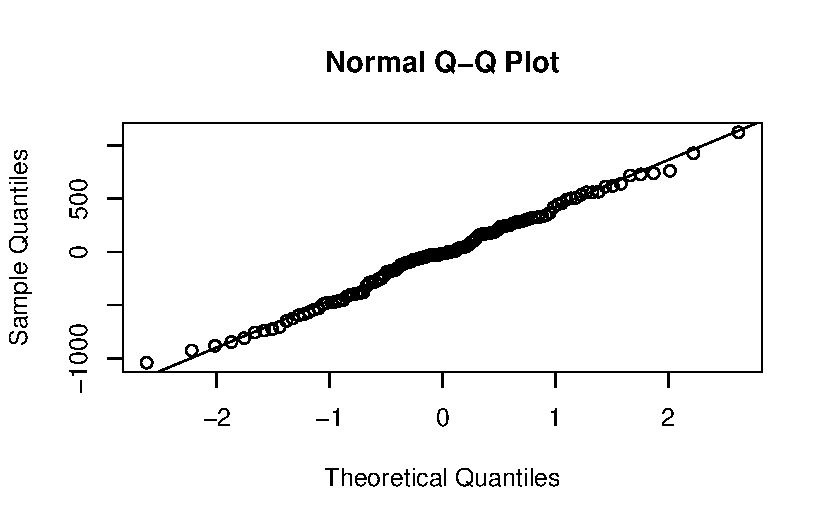
\includegraphics{T2_grupo10_files/figure-pdf/unnamed-chunk-2-1.pdf}

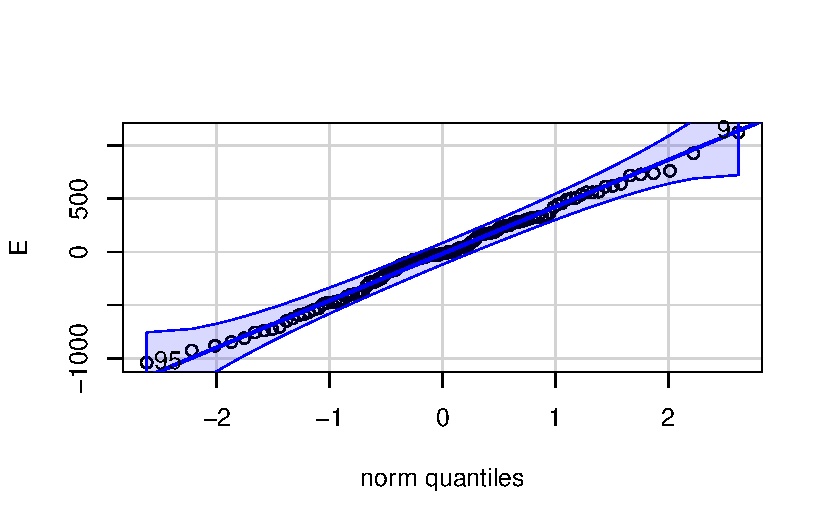
\includegraphics{T2_grupo10_files/figure-pdf/unnamed-chunk-2-2.pdf}

\begin{verbatim}
[1]  9 95
\end{verbatim}

\begin{verbatim}

    Shapiro-Wilk normality test

data:  E
W = 0.99331, p-value = 0.8598
\end{verbatim}

\begin{verbatim}

    Box-Ljung test

data:  E
X-squared = 12.639, df = 20, p-value = 0.8923
\end{verbatim}

\begin{verbatim}
       ar1        ar2       sma1 
-0.5096443 -0.3354277 -0.5080884 
\end{verbatim}

\begin{verbatim}
[1] 189154.6
\end{verbatim}

Assim, pela imagem, com envelope de 95\%, é basicamente certa a
normalidade dos resíduos, para confirmar, é conduzido o teste de
Shapiro-Wilk, sob hipóteses:

\begin{align}
  \begin{cases}
    H_0:\text{Os resíduos seguem distribuição normal}\\
    H_1: \text{Os resíduos não seguem distribuição normal}\\
  \end{cases}
\end{align}

Assim, com nível de significância de 5\%, o teste de Shapiro-Wilk
confirma que os resíduos estão distribuidos segundo uma distribuição
normal.

\hypertarget{com-transformauxe7uxe3o-de-box-cox}{%
\subsection{Com transformação de
Box-Cox}\label{com-transformauxe7uxe3o-de-box-cox}}

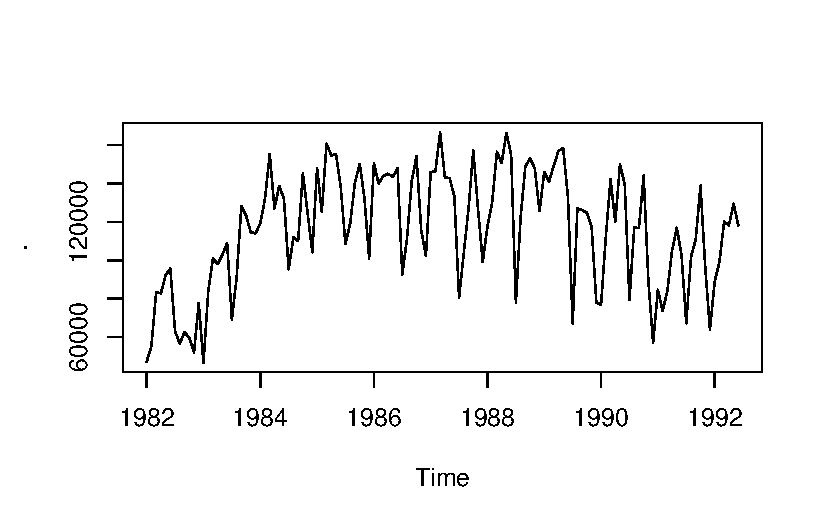
\includegraphics{T2_grupo10_files/figure-pdf/unnamed-chunk-3-1.pdf}

Percebe-se grande similaridade com a série original, e, pode-se
prosseguir da mesma maneira que anteriormente com o procedimento de
seleção. Primeiramente, testando a estacionariedade da série com o teste
KPSS a un nível de significância de 5\%, é possível concluir que a série
não é estacionária (p-valor = 0, 03658). Dessa maneira, analogamente à
análise da série sem a transformação Box-Cox, é necessário aplicar 1
diferenciação simples e de uma diferenciação sazonal para tornar a série
estácionária, sendo d = 1 e D = 1. Da mesma maneira que na análise
anterior, foi utilizado um sazonal de 12 para a diferenciação sazonal,
dessa maneira, a série diferenciada é a que se segue:

\begin{verbatim}

    KPSS Test for Level Stationarity

data:  x2
KPSS Level = 0.5226, Truncation lag parameter = 4, p-value = 0.03658
\end{verbatim}

\begin{verbatim}
[1] 1
\end{verbatim}

\begin{verbatim}
[1] 1
\end{verbatim}

\begin{verbatim}
Series: x2 
ARIMA(0,1,1)(0,1,1)[12] 

Coefficients:
          ma1     sma1
      -0.5166  -0.5532
s.e.   0.0825   0.1060

sigma^2 = 238912745:  log likelihood = -1251.65
AIC=2509.31   AICc=2509.53   BIC=2517.49
\end{verbatim}

\begin{verbatim}

    KPSS Test for Level Stationarity

data:  diff_bc
KPSS Level = 0.044088, Truncation lag parameter = 4, p-value = 0.1
\end{verbatim}

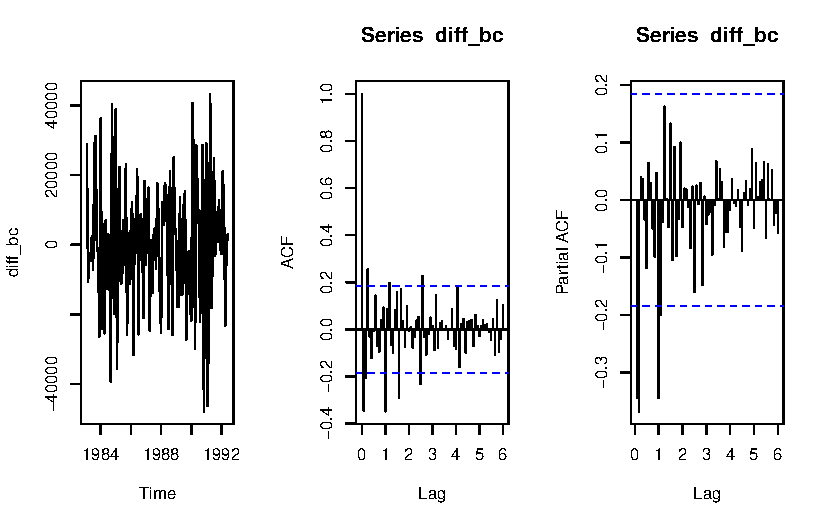
\includegraphics{T2_grupo10_files/figure-pdf/unnamed-chunk-5-1.pdf}

Assim ficou a série a partir de 1 diferenciação simples e sazonal.
Agora, analogamente à série sem transformação, é possível observar que a
série tem aparência estacionária, o que deve ser confirmado novamente a
partir do teste de KPSS de sob hipóteses já explicitadas. Assim, a
partir de um p-valor maior que 0.1, pôde-se confirmar que a série
diferenciada é estacionária e que é possível prosseguir com o
procedimento de seleção.

\begin{verbatim}
p = 0 , d = 1, q = 0 , P =  0 , D = 1, Q =  0 , AICc = 2553.741 
p = 0 , d = 1, q = 1 , P =  0 , D = 1, Q =  0 , AICc = 2531.436 
p = 0 , d = 1, q = 3 , P =  0 , D = 1, Q =  0 , AICc = 2531.137 
p = 1 , d = 1, q = 2 , P =  0 , D = 1, Q =  0 , AICc = 2530.789 
p = 2 , d = 1, q = 0 , P =  0 , D = 1, Q =  0 , AICc = 2526.922 
p = 0 , d = 1, q = 1 , P =  0 , D = 1, Q =  1 , AICc = 2509.529 
p = 2 , d = 1, q = 0 , P =  0 , D = 1, Q =  1 , AICc = 2506.5 
\end{verbatim}

\begin{verbatim}
[1] 2506.5
\end{verbatim}

Assim, pode-se observar comportamento similar ao da série sem a
transformação de Boxcox. Nesse sentido, no gráfico ACF há uma quebra no
primeiro lag simples, ao passo que há uma quebra no segundo lag no
gráfico PACF. Nenhum dos gráficos apresentou comportamento bem
definido.Para os lags sazonais, percebem-se valores significativos
apenas no primeiro lag, sendo assim, os valores de p e q serão testados
entre 0 e 2, já P e Q, nos valores 0 ou 1, desconsiderando quando p e q
forem 0 simultaneamente, e analogamente para P e Q. A partir dos AICc,
observou-se o melhor menor valor de 2506, 5 e assim, o modelo ajustado
foi um SARIMA\((2, 1, 0)(0, 1, 1)_{12}\), assim com no ajuste de modelo
sem utilização da transformação de Box-Cox.

Seguindo para análise dos resíduos, é possível observar que há uma
sequência de resíduos iguais a zero no início da série.

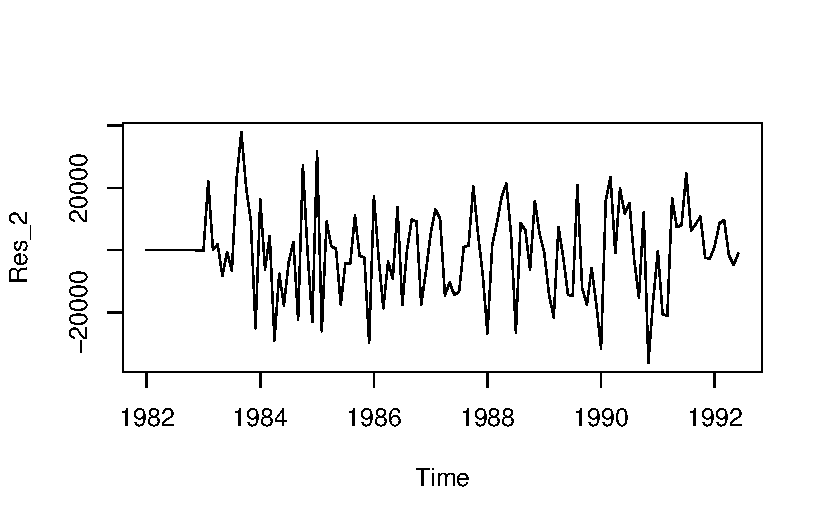
\includegraphics{T2_grupo10_files/figure-pdf/unnamed-chunk-7-1.pdf}

Assim, analogamente à série sem transformação, serão considerados apenas
os resíduos um ano após o início das observações, dados pela figura a
seguir:

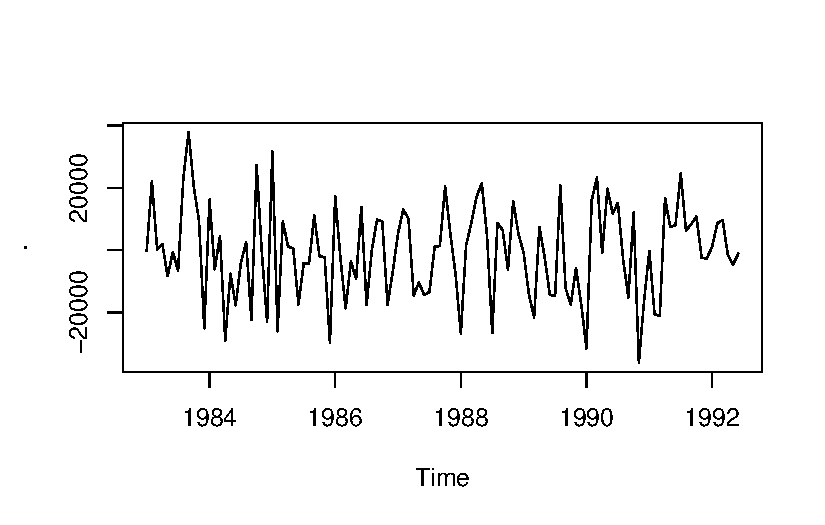
\includegraphics{T2_grupo10_files/figure-pdf/unnamed-chunk-8-1.pdf}

Analisando graficamente, os residuos aparentam estacionariedade, mas
para testar se essa suspeita é correta, utiliza-se o teste de KPSS. O
teste mostra que os resíduos são, de fato, estácionários (p-valor
\textgreater{} 0, 1). Além disso, pode-se visualizar pelo gráfico do
ACF, a independência dos resíduos:

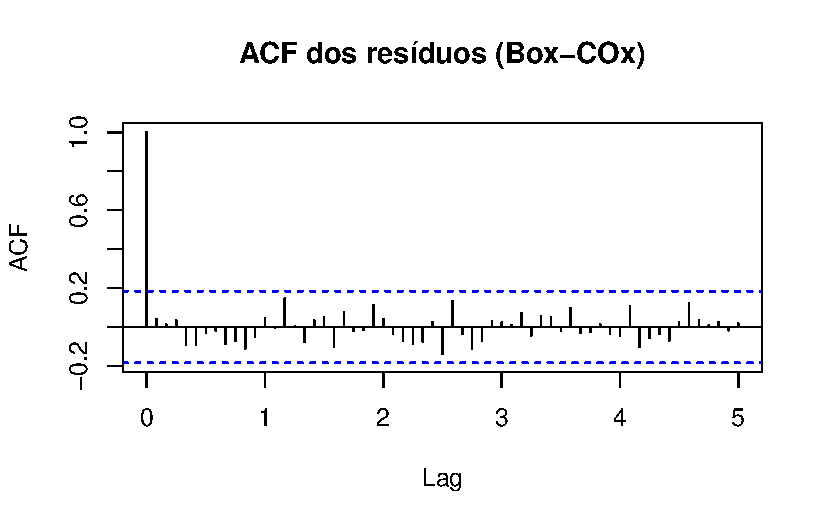
\includegraphics{T2_grupo10_files/figure-pdf/unnamed-chunk-9-1.pdf}

Assim, de maneira análoga à vista na série sem transformação de Box-Cox,
basicamente não há valores significativos, e, para realmente confirmar
independência, utiliza-se novamente o teste do tipo Ljung-Box. Assim,
com 20 graus de liberdade, o p-valor foi de 0, 86, e com 15 graus, o
p-valor resultou em 0.8443, portanto, para um nível de significância de
5\%, não se rejeita H0, indicando que a suspeita após a análise gráfica
estava correta, e os resíduos realmente são independentes. Por fim,
pode-se prosseguir com a análise da normalidade dos resíduos, por meio
da análise gráfica primeiramente.

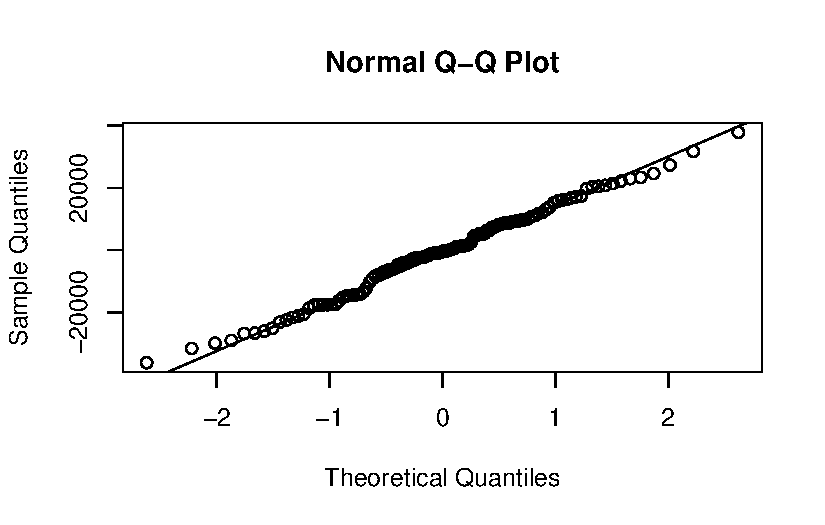
\includegraphics{T2_grupo10_files/figure-pdf/unnamed-chunk-10-1.pdf}

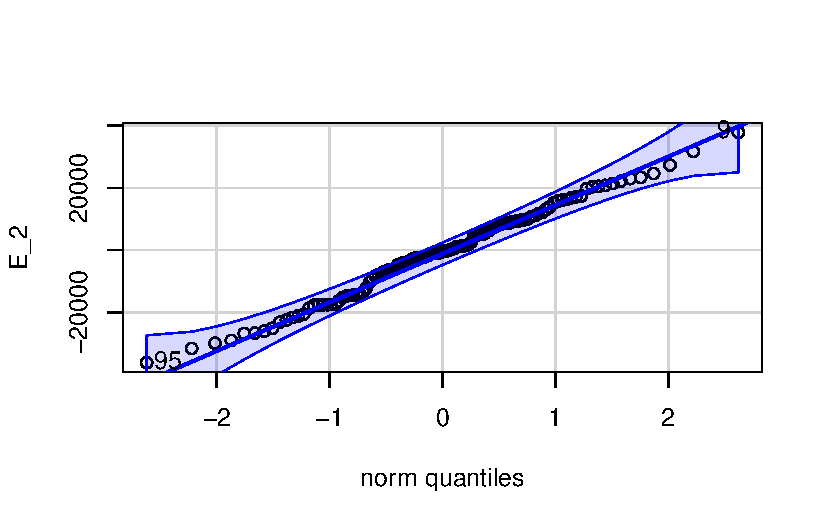
\includegraphics{T2_grupo10_files/figure-pdf/unnamed-chunk-10-2.pdf}

\begin{verbatim}
[1]  9 95
\end{verbatim}

\begin{verbatim}

    Shapiro-Wilk normality test

data:  E_2
W = 0.99199, p-value = 0.7513
\end{verbatim}

\begin{verbatim}

    KPSS Test for Level Stationarity

data:  E_2
KPSS Level = 0.062576, Truncation lag parameter = 4, p-value = 0.1
\end{verbatim}

\begin{verbatim}

    Box-Ljung test

data:  E_2
X-squared = 13.39, df = 20, p-value = 0.86
\end{verbatim}

\begin{verbatim}
       ar1        ar2       sma1 
-0.5059202 -0.3433980 -0.5264162 
\end{verbatim}

\begin{verbatim}
[1] 224602516
\end{verbatim}

A partir da análise gráfica, é possível observar indicação de
normalidade dos resíduos. Seguindo com o teste de Shapiro-Wilk, há
evidências de que os resíduos seguem distribuição normal (p-valor=0,
7513).

\hypertarget{modelos-ets-seleuxe7uxe3o-transformauxe7uxf5es-e-resuxedduos}{%
\section{Modelos ETS: seleção, transformações e
resíduos}\label{modelos-ets-seleuxe7uxe3o-transformauxe7uxf5es-e-resuxedduos}}

Modelos ETS tem uma estrutura que perite descrever os modelos de
alisamento exponecial em função dos tipos das suas componentes, sendo
elas: erro, tendência e sazonalidade. Nesses modelos a tendência pode
ser de 5 tipos, sendo: sem tendência, com tendência aditiva, com
tendência aditiva mais damped, com tendência multiplicativa e com
tendência multiplicativa mais damped. Já a sazonalidade pode ser de 3
tipos: sem sazonalidade, com sazonalidade atitiva e com sazonalidade
multiplicativa. Combinar os tipos diferentes de tendência com os tipos
diferentes de sazonalidade, resulta em 15 tipos diferentes de modelos
que posem ser ajustados. Em adição, o termo de erro pode ser incluido de
maneira aditiva ou de maneira multiplicativa, resultando em um total de
30 modelos possíveis.

\begin{longtable*}{lccc}
\toprule
Modelo & AIC & AICc & BIC\\
\midrule
\endfirsthead
\multicolumn{4}{@{}l}{\textit{(continued)}}\\
\toprule
Modelo & AIC & AICc & BIC\\
\midrule
\endhead

\endfoot
\bottomrule
\endlastfoot
\cellcolor{gray!15}{ETS(A,Ad,A)} & \cellcolor{gray!15}{2154.36} & \cellcolor{gray!15}{2160.76} & \cellcolor{gray!15}{2205.42}\\
ETS(A,A,A) & 2157.50 & 2163.17 & 2205.72\\
\cellcolor{gray!15}{ETS(A,N,A)} & \cellcolor{gray!15}{2162.35} & \cellcolor{gray!15}{2166.71} & \cellcolor{gray!15}{2204.89}\\
ETS(M,Ad,M) & 2179.42 & 2185.81 & 2230.47\\
\cellcolor{gray!15}{ETS(M,M,M)} & \cellcolor{gray!15}{2181.29} & \cellcolor{gray!15}{2187.68} & \cellcolor{gray!15}{2232.34}\\
ETS(M,A,M) & 2184.06 & 2189.72 & 2232.27\\
\cellcolor{gray!15}{ETS(M,M,M)} & \cellcolor{gray!15}{2192.25} & \cellcolor{gray!15}{2197.92} & \cellcolor{gray!15}{2240.47}\\
ETS(M,Ad,A) & 2194.14 & 2200.54 & 2245.20\\
\cellcolor{gray!15}{ETS(M,A,A)} & \cellcolor{gray!15}{2196.12} & \cellcolor{gray!15}{2201.79} & \cellcolor{gray!15}{2244.34}\\
ETS(M,N,M) & 2196.41 & 2200.78 & 2238.96\\*
\end{longtable*}

Após varredura dos modelos ETS possíveis, o modelo com menor AICc
selecionado foi um ETS\((A, A_{d}, A)\), ou seja, um modelo ETS com
sazonalidade aditiva, tendência aditiva com damped e erro aditivo. A
decomposição da série pode ser observada no gráfico abaixo.

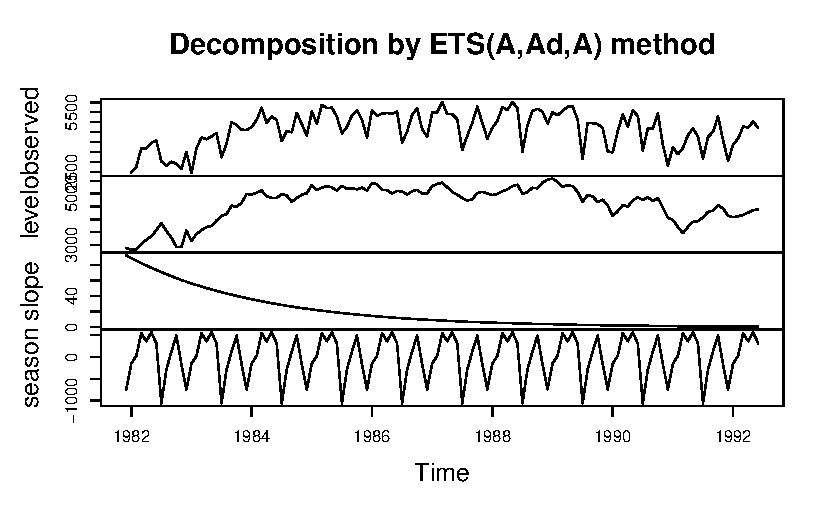
\includegraphics{T2_grupo10_files/figure-pdf/melhor-fit-ETL-sem-transf-1.pdf}

\hypertarget{resuxedduos}{%
\subsubsection{Resíduos}\label{resuxedduos}}

Seguindo com a análise de resíduos do modelo ajustado, observa-se os
seguintes resultados.

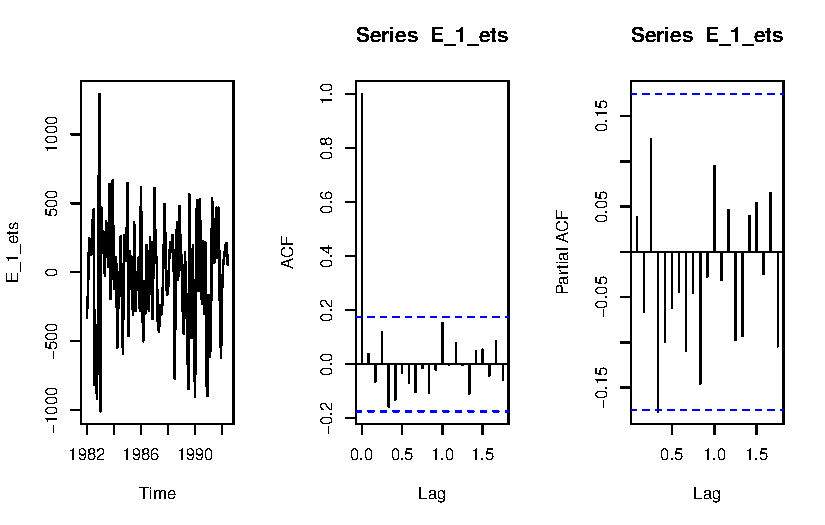
\includegraphics{T2_grupo10_files/figure-pdf/residuos-ets-sem-transform-1.pdf}

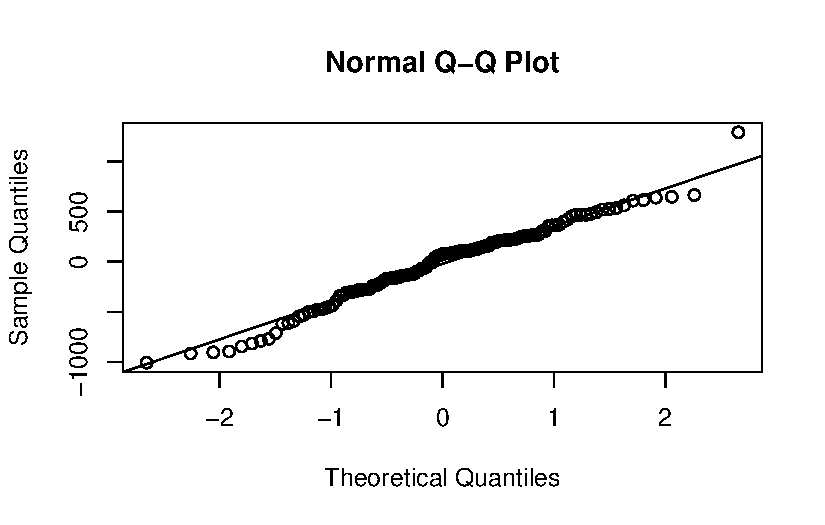
\includegraphics{T2_grupo10_files/figure-pdf/residuos-ets-sem-transform-2.pdf}

Analisando graficamente, os residuos aparentam estacionariedade.
Aplicando o teste de KPSS é posspivel observar que, de fato, os resíduos
são estácionários (p-valor \textgreater{} 0, 1). Além disso, pode-se
visualizar pelo gráfico do ACF, a independência dos resíduos.

\begin{verbatim}

    KPSS Test for Level Stationarity

data:  E_1_ets
KPSS Level = 0.064386, Truncation lag parameter = 4, p-value = 0.1
\end{verbatim}

\begin{verbatim}

    Box-Ljung test

data:  E_1_ets
X-squared = 16.069, df = 15, p-value = 0.3775
\end{verbatim}

\begin{verbatim}

    Shapiro-Wilk normality test

data:  E_1_ets
W = 0.98013, p-value = 0.06068
\end{verbatim}

\begin{tabular}{l|r|r}
\hline
  & Estatistica & p\_valor\\
\hline
W & 0.9801266 & 0.0606769\\
\hline
KPSS Level & 0.0643859 & 0.1000000\\
\hline
X-squared & 16.0693204 & 0.1880817\\
\hline
\end{tabular}

Seguindo para os teste de independência e normalidade dos resíduos, é
possível concluir que eles são independentes (p-valor = 0,188) e estão
normalmente distribuídos (p-valor = 0,061), a um nível de significância
de 5\%. No entanto, especificamente para o teste de normalidade, não se
pode dizer que é um teste muito confiável, já que alterar o nível de
significância pode alterar o resultado do teste.

\hypertarget{modelo-com-transformauxe7uxe3o}{%
\subsection{Modelo com
transformação}\label{modelo-com-transformauxe7uxe3o}}

\hypertarget{seleuxe7uxe3o}{%
\subsubsection{Seleção}\label{seleuxe7uxe3o}}

Para a seleção de um modelo utilisando a transformação de Box-Cox,
primeiramente sou definido o valor de \(\lambda\) que melhor se
ajustasse a série, sendo esse valor de \(\lambda = 1,422\), como pode
ser observado no gráfico abaixo.

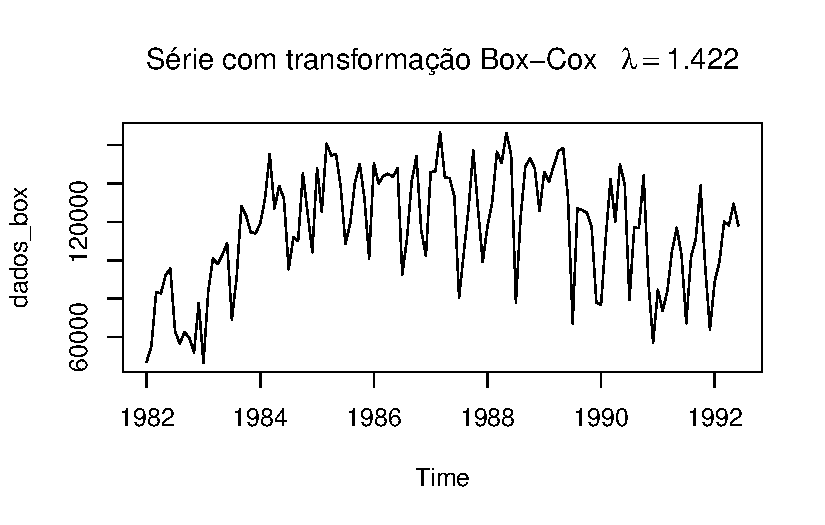
\includegraphics{T2_grupo10_files/figure-pdf/ETS-com-transf-1.pdf}

Seguindo o mesmo procedimento aplicado para selecionar o modelo sem
transformação de Box-Cox, foi feita uma varreura de todos os modelos
possíveis e o melhor deles foi selecionado segundo o critério AICc.

\begin{longtable*}{lccc}
\toprule
Modelo transformado & AIC & AICc & BIC\\
\midrule
\endfirsthead
\multicolumn{4}{@{}l}{\textit{(continued)}}\\
\toprule
Modelo transformado & AIC & AICc & BIC\\
\midrule
\endhead

\endfoot
\bottomrule
\endlastfoot
\cellcolor{gray!15}{ETS(A,Ad,A)} & \cellcolor{gray!15}{3044.31} & \cellcolor{gray!15}{3050.71} & \cellcolor{gray!15}{3095.37}\\
ETS(A,A,A) & 3047.45 & 3053.12 & 3095.67\\
\cellcolor{gray!15}{ETS(A,N,A)} & \cellcolor{gray!15}{3049.98} & \cellcolor{gray!15}{3054.35} & \cellcolor{gray!15}{3092.53}\\
ETS(M,Ad,M) & 3072.16 & 3078.55 & 3123.21\\
\cellcolor{gray!15}{ETS(M,M,M)} & \cellcolor{gray!15}{3073.43} & \cellcolor{gray!15}{3079.82} & \cellcolor{gray!15}{3124.49}\\
ETS(M,A,M) & 3079.96 & 3085.63 & 3128.18\\
\cellcolor{gray!15}{ETS(M,M,M)} & \cellcolor{gray!15}{3086.13} & \cellcolor{gray!15}{3091.80} & \cellcolor{gray!15}{3134.35}\\
ETS(M,N,M) & 3087.88 & 3092.24 & 3130.42\\
\cellcolor{gray!15}{ETS(M,Ad,A)} & \cellcolor{gray!15}{3101.83} & \cellcolor{gray!15}{3108.22} & \cellcolor{gray!15}{3152.88}\\
ETS(M,A,A) & 3108.98 & 3114.65 & 3157.20\\*
\end{longtable*}

O modelo selecionado segundo o menor AICc, levando em consideração a
transformação de Box-Cox, foi o mesmo selecionado anteriormente, sendo
ETS\((A, A_{d}, A)\), ou seja, um modelo ETS com sazonalidade aditiva,
tendência aditiva com damped e erro aditivo.

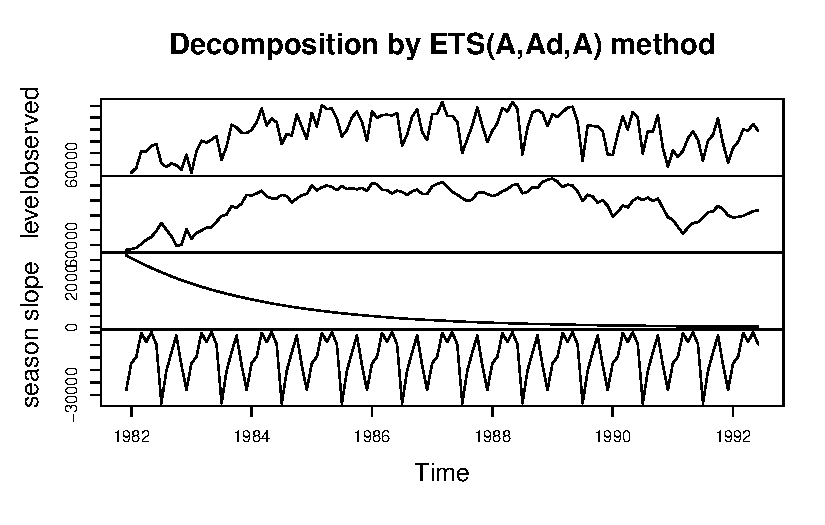
\includegraphics{T2_grupo10_files/figure-pdf/melhor-fit-ETL-com-transf-1.pdf}

\hypertarget{resuxedduos-1}{%
\subsubsection{Resíduos}\label{resuxedduos-1}}

\includegraphics{T2_grupo10_files/figure-pdf/resíduos-modelo-transformado-1.pdf}

\includegraphics{T2_grupo10_files/figure-pdf/resíduos-modelo-transformado-2.pdf}

Analisando graficamente, os residuos aparentam estacionariedade.
Aplicando o teste de KPSS é posspivel observar que, de fato, os resíduos
são estácionários (p-valor \textgreater{} 0, 1). Além disso, pode-se
visualizar pelo gráfico do ACF, a independência dos resíduos.

\begin{verbatim}

    KPSS Test for Level Stationarity

data:  E_2_ets
KPSS Level = 0.071953, Truncation lag parameter = 4, p-value = 0.1
\end{verbatim}

\begin{verbatim}

    Box-Ljung test

data:  E_2_ets
X-squared = 15.575, df = 15, p-value = 0.4109
\end{verbatim}

\begin{verbatim}

    Shapiro-Wilk normality test

data:  E_2_ets
W = 0.98338, p-value = 0.1257
\end{verbatim}

\begin{tabular}{l|r|r}
\hline
  & Estatistica & p\_valor\\
\hline
W & 0.9833828 & 0.1256580\\
\hline
KPSS Level & 0.0719535 & 0.1000000\\
\hline
X-squared & 15.5745517 & 0.2115083\\
\hline
\end{tabular}

Seguindo para os teste de independência e normalidade dos resíduos, é
possível concluir que eles são independentes (p-valor = 0,4109) e estão
normalmente distribuídos (p-valor = 0,1257), a um nível de significância
de 5\%. Nesse caso, tanto o teste de independência quanto o teste de
normalidade tem resultados mais confiáveis.

\hypertarget{estudo-de-desempenho-preditivo}{%
\section{Estudo de desempenho
preditivo}\label{estudo-de-desempenho-preditivo}}

\hypertarget{resultados-da-janela-deslizante}{%
\subsection{Resultados da Janela
Deslizante}\label{resultados-da-janela-deslizante}}

\hypertarget{performance-em-relauxe7uxe3o-aos-horizontes-de-previsuxe3o}{%
\subsection{Performance em relação aos horizontes de
previsão}\label{performance-em-relauxe7uxe3o-aos-horizontes-de-previsuxe3o}}

\hypertarget{arima}{%
\subsubsection{ARIMA}\label{arima}}

\hypertarget{ets}{%
\subsubsection{ETS}\label{ets}}

\hypertarget{resultados}{%
\section{Resultados}\label{resultados}}

apresente em tabelas e gráficos as previsões dos 4 modelos selecionados
e também apresente em uma tabela os resultados de acurácia dos 4 modelos
selecionados e dos modelos benchmarks. Comente os resultados de modo
objetivo;

\hypertarget{apuxeandice}{%
\section{Apêndice}\label{apuxeandice}}

Todo o projeto de composição deste documento pode ser encontrado aqui:
https://github.com/cesar-galvao/trabalhos\_series



\end{document}
